\chapter{Specifikacija programske potpore}
		
	\section{Funkcionalni zahtjevi}
			
	    	\noindent \textbf{Dionici:}
			
			\begin{packed_enum}
				
				\item Vlasnik (naručitelj)
				\item Pacijenti
				\item Zdravstveni djelatnici			
				\item Administrator
				\item Razvojni tim
				
			\end{packed_enum}
			
			
			\noindent \textbf{Aktori i njihovi funkcionalni zahtjevi:}
			
			
			\begin{packed_enum}
				\item  \underbar{Neregistrirani/neprijavljeni korisnik (inicijator) može:}
				
				\begin{packed_enum}
					
					\item se registrirati u sustav kao pacijent te tako stvoriti novi korisnički račun za koji su mu potrebni ime, prezime, e-mail adresa, OIB i lozinka
					\item pregledati naslovnu stranicu i stranicu koja objašnjava funkcionalnost aplikacije
					
					
				\end{packed_enum}
			
				\item  \underbar{Pacijent (inicijator) može:}
				
				\begin{packed_enum}
					
					\item prijaviti se u sustav
					\item odabrati željeni termin dolazaka, a ukoliko se radi o ponovljenoj terapiji i referencu na već obavljeni postupak terapije u ustanovi
					\item navesti opis svog oboljenja te odabrati liječnika koji će ga liječiti
					\item otkazati zakazani termin u roku 24 sata prije samoga termina te potvrditi ili odbiti pomaknuti termin zbog novonastale okolnosti
					\item primati elektroničku poštu o zakazanom terminu i novonastalim okolnostima
					
				\end{packed_enum}
			
			
			\item  \underbar{Zdravstveni djelatnik (inicijator) može:}
			
			\begin{packed_enum}
				
				\item prijaviti se u sustav
				\item pregledavati prijave i dodjeljivati pacijentima termine
				\item direktno kontaktirati pacijenta putem elektroničke pošte u slučaju neočekivanih promjena
				\item vidjeti sve pacijente i sve tretmane koji su im dodijeljeni
				\item nakon obavljenog postupka rehabilitacije registrirati dolazak pacijenta
				\item nakon završenog ciklusa upisati postignute rezultate s pacijentom
				
				
			\end{packed_enum}
			
			
			\item  \underbar{Administrator (inicijator) može:}
			
			\begin{packed_enum}
				
				\item verificirati podatke iz središnjeg informacijskog sustava zdravstvene zaštite
				\item pristupiti popisu korisnika, zdravstvenih djelatnika te njihovim osobnim podacima
				\item stvoriti zdravstvenog djelatnika u sustavu
				
			\end{packed_enum}
			
			\item  \underbar{Baza podataka (sudionik) može:}
			
			\begin{packed_enum}
				
				\item pohraniti podatke o korisnicima i njihovim dopuštenjima
				\item pohraniti podatke o terminima (slobodnim i zauzetim)
				\item pohraniti podatke o opremama/uslugama (slobodnim i zauzetim)
				
			\end{packed_enum}
		\end{packed_enum}
			
			\eject 
			
			
				
			\subsection{Obrasci uporabe}
	

					\noindent \underbar{\textbf{UC1 - Registracija}}
					\begin{packed_item}
	
						\item \textbf{Glavni sudionik: }Korisnik
						\item  \textbf{Cilj:} Stvoriti korisnički račun za pacijenta
						\item  \textbf{Sudionici:} Baza podataka
						\item  \textbf{Preduvjet:} -
						\item  \textbf{Opis osnovnog tijeka:}
						
						\item[] \begin{packed_enum}
	
							\item Korisnik odabire opciju za registriranje
							\item Korisnik unosi potrebne podatke
							\item Korisnik pritišće dugme da potvrdi registraciju
							\item Korisnik prima obavijest o uspješnoj registraciji
						\end{packed_enum}
						
						\item  \textbf{Opis mogućih odstupanja:}
						
						\item[] \begin{packed_item}
	
							\item[2.a] Odabir zauzetog e-maila i/ili korisničkog imena, unos neispravnog e-maila, unos korisničkog podatka u zabranjenom formatu ili pogrešno napisana ponovljena lozinka (polje "Potvrdi lozinku")
							\item[] \begin{packed_enum}
								
								\item Korisnik dobiva obavijest o neuspješnoj registraciji i vraća ga na stranicu za registraciju
								\item Korisnik mijenja krivo unešene podatke ili odustaje od registracije
								
							\end{packed_enum}
							
						\end{packed_item}
					\end{packed_item}
					
					\noindent \underbar{\textbf{UC2 - Prijava u sustav}}
					\begin{packed_item}
						
						\item \textbf{Glavni sudionik: }Pacijent
						\item  \textbf{Cilj:} Pristupiti uslugama koje pruža naš sustav
						\item  \textbf{Sudionici:} Baza podataka
						\item  \textbf{Preduvjet:} Registracija u sustav
						\item  \textbf{Opis osnovnog tijeka:}
						
						\item[] \begin{packed_enum}
							
							\item Pacijent odabire opciju za prijavu
							\item Pacijent unosi korisničko ime i lozinku
							\item Pacijent pritišće dugme da potvrdi prijavu
							\item Pacijent pristupa uslugama za koje ima dopuštenje 
						\end{packed_enum}
						
						\item  \textbf{Opis mogućih odstupanja:}
						
						\item[] \begin{packed_item}
							
							\item[2.a] Neispravno korisničko ime i/ili lozinka
							\item[] \begin{packed_enum}
								
								\item Korisnik dobiva obavijest o neuspješnoj prijavi i vraća ga na stranicu za prijavu
								\item Korisnik mijenja krivo unešene podatke ili odustaje od prijave (vraća se na naslovnu stranu)
								
							\end{packed_enum}
							
						\end{packed_item}
					\end{packed_item}
					
					\noindent \underbar{\textbf{UC3 - Upravljanje terminima}}\\
					\textit{Uključuje obrasce uporabe UC3.1. Zakazivanje termina, UC3.2. Otkazivanje termina, UC3.3. Pregled termina i UC3.4 Potvrđivanje novih termina.}\\
					
					\noindent \underbar{\textbf{UC3.1. - Zakazivanje termina}}
					\begin{packed_item}
						
						\item \textbf{Glavni sudionik: }Pacijent
						\item  \textbf{Cilj:} Mogućnost odabira termina za odlazak na fizikalnu terapiju
						\item  \textbf{Sudionici:} Baza podataka
						\item  \textbf{Preduvjet:} Korisnik prijavljen kao pacijent
						\item  \textbf{Opis osnovnog tijeka:}
						
						\item[] \begin{packed_enum}
							
							\item Pacijent odabire opciju za zakazivanje termina
							\item Pacijent na prikazanom kalendaru izabire poželjni slobodni termin
							\item Pacijent navodi vrstu i opis oboljenja, zahtijevani postupak liječenja i liječnika koji ih je uputio
							\item Ako se radi o ponovljenoj terapiji, pacijent odabire referencu na već obavljeni postupak terapije
							\item Pacijent pritišće dugme za potvrdu odabranog termina
							\item Pacijent dobiva e-mail potvrdu o odabranom terminu
						\end{packed_enum}
						
						\item  \textbf{Opis mogućih odstupanja:}
						
						\item[] \begin{packed_item}
							
							\item[2.a] Pacijent se nije pojavio na zakazanom terminu
							\item[] \begin{packed_enum}
								
								\item Pacijent dobiva e-mail poruku upozorenja da sljedeći put ako se ponovi će dobiti zabranu zakazivanja termina
								
							\end{packed_enum}
							
							\item[2.b] Pacijent se nije pojavio na zakazanom terminu drugi put
							\item[] \begin{packed_enum}
								
								\item Pacijentu se zabranjuje zakazivanje termina na određeno vrijeme te dobiva tu obavijest na e-mailu
								
							\end{packed_enum}
							
							\item[2.c] Pacijent je zakazao 3 termina u istom tjednu
							\item[] \begin{packed_enum}
								
								\item Pacijentu se zabranjuje zakazivanje više od 2 termina tjedno te bude u tome onemogućen
								
							\end{packed_enum}
							
						\end{packed_item}
					\end{packed_item}
					
					\noindent \underbar{\textbf{UC3.2. - Otkazivanje termina}}
					\begin{packed_item}
						
						\item \textbf{Glavni sudionik: }Pacijent
						\item  \textbf{Cilj:} Mogućnost otkazivanja termina 
						\item  \textbf{Sudionici:} Baza podataka
						\item  \textbf{Preduvjet:} Korisnik prijavljen kao pacijent i ima zakazan određen termin
						\item  \textbf{Opis osnovnog tijeka:}
						
						\item[] \begin{packed_enum}
							
							\item Pacijent odabire opciju za zakazivanje termina
							\item Pacijent na kalendaru odabire zakazani termin koji želi otkazati
							\item Pacijent odabire opciju za otkazivanje odabranog termina
							\item Pacijent pritišće dugme za potvrdu otkazivanja termina
							\item Pacijent dobiva e-mail potvrdu o otkazanom terminu
						\end{packed_enum}
						
						\item  \textbf{Opis mogućih odstupanja:}
						
						\item[] \begin{packed_item}
							
							\item[3.a] Pacijent prekasno pokušava otkazati termin (24 sata prije zakazanog termina)
							\item[] \begin{packed_enum}
								
								\item Sustav onemogućuje pacijentu otkazivanje tog termina
								
							\end{packed_enum}
							
						\end{packed_item}
					\end{packed_item}
					
					\noindent \underbar{\textbf{UC3.3. - Pregled termina}}
					\begin{packed_item}
						
						\item \textbf{Glavni sudionik: }Pacijent
						\item  \textbf{Cilj:} Mogućnost prikaza zakazanih termina
						\item  \textbf{Sudionici:} Baza podataka
						\item  \textbf{Preduvjet:} Korisnik prijavljen kao pacijent
						\item  \textbf{Opis osnovnog tijeka:}
						
						\item[] \begin{packed_enum}
							
							\item Pacijent na kalendaru može vidjeti svoje zakazane termine
						\end{packed_enum}
					\end{packed_item}
					
						\noindent \underbar{\textbf{UC3.4. - Potvrđivanje novih termina}}
					\begin{packed_item}
						
						\item \textbf{Glavni sudionik: }Pacijent
						\item  \textbf{Cilj:} Mogućnost prihvaćanja ili odbijanja novog termina (zbog novonastale okolnosti)
						\item  \textbf{Sudionici:} Baza podataka
						\item  \textbf{Preduvjet:} Korisnik prijavljen kao pacijent, zdravstveni djelatnik je predložio pomak termina iz raznih razloga (npr. nedostajanje opreme za tretman)
						\item  \textbf{Opis osnovnog tijeka:}
						
						\item[] \begin{packed_enum}
							
							\item Pacijent dobiva e-mail obavijest o pomaku termina
							\item Pacijent u posebnom prozoru dobiva uvid o kojem novom terminu se radi
							\item Pacijent odabire prihvaća li ili ne novi navedeni termin
							\item Pacijent pritišće dugme kako bi potvrdio svoju odluku
							\item Pacijent dobiva e-mail potvrdu da je sustav zaprimio njegovu odluku (prihvaćanje ili odbijanje termina)
						\end{packed_enum}
					\end{packed_item}
					
					\noindent \underbar{\textbf{UC4 - E-mail podsjetnik za termin}}
					\begin{packed_item}
						
						\item \textbf{Glavni sudionik: }-
						\item  \textbf{Cilj:} Slanje e-mail podsjetnik za zakazani termin (24 sata prije termina)
						\item  \textbf{Sudionici:} Baza podataka, pacijent
						\item  \textbf{Preduvjet:} Korisnik prijavljen kao pacijent i postoji zakazani termin
						\item  \textbf{Opis osnovnog tijeka:}
						
						\item[] \begin{packed_enum}
							
							\item Pacijent dobiva e-mail obavijest o zakazanom terminu
						\end{packed_enum}
					\end{packed_item}
					
					\noindent \underbar{\textbf{UC5 - Kontrola slobodnih/zauzetih termina}}
					\begin{packed_item}
						
						\item \textbf{Glavni sudionik: }Zdravstveni djelatnik
						\item  \textbf{Cilj:} Omogućiti na vrijeme odrediti koji termini su slobodni za fizikalnu terapiju i medicinsku rehabilitaciju (ovisi o količini dostupne opreme/usluge, kapacitetu prostorija i radnom vremenu ustanove)
						\item  \textbf{Sudionici:} Baza podataka
						\item  \textbf{Preduvjet:} Korisnik prijavljen kao zdravstveni djelatnik
						\item  \textbf{Opis osnovnog tijeka:}
						
						\item[] \begin{packed_enum}
							
							\item Zdravstveni djelatnik bira opciju za uređivanje termina, odnosno postavljanje termina zauzetim ili dostupnim
							\item Zdravstveni djelatnik pritiskom na dostupno dugme sprema novonastale promjene
						\end{packed_enum}
					\end{packed_item}
					
					\noindent \underbar{\textbf{UC6 - Pregled svojih rezerviranih termina}}
					\begin{packed_item}
						
						\item \textbf{Glavni sudionik: }Zdravstveni djelatnik
						\item  \textbf{Cilj:} Omogućiti zdravstvenom djelatniku pregled termina koji su rezervirali isključivo njegovi pacijenti
						\item  \textbf{Sudionici:} Baza podataka
						\item  \textbf{Preduvjet:} Korisnik prijavljen kao zdravstveni djelatnik
						\item  \textbf{Opis osnovnog tijeka:}
						
						\item[] \begin{packed_enum}
							
							\item Zdravstveni djelatnik na kalendaru može vidjeti za pojedini dan koji su mu termini rezervirani
						\end{packed_enum}
					\end{packed_item}

					
					\noindent \underbar{\textbf{UC6.1. - Pomicanje svojih rezerviranih termina}}
					\begin{packed_item}
						
						\item \textbf{Glavni sudionik: }Zdravstveni djelatnik
						\item  \textbf{Cilj:} Omogućiti zdravstvenom djelatniku da pomakne rezervirani termin zbog novonastale okolnosti te čeka potvrdu ili odbijanje od strane pacijenta (to ne smije činiti u istom danu kada je taj termin zakazan, mora biti na vrijeme organiziran)
						\item  \textbf{Sudionici:} Baza podataka
						\item  \textbf{Preduvjet:} Korisnik prijavljen kao zdravstveni djelatnik
						\item  \textbf{Opis osnovnog tijeka:}
						
						\item[] \begin{packed_enum}
							
							\item Zdravstveni djelatnik na kalendaru odabire zakazani termin koji želi pomaknuti
							\item Zdravstveni djelatnik bira opciju za otkazivanje tog termina i predlaže pacijentu novi termin
							\item Zdravstveni djelatnik pritiskom na dugme potvrđuje promjenu termina
						\end{packed_enum}
						
						\item  \textbf{Opis mogućih odstupanja:}
						
						\item[] \begin{packed_item}
							
							\item[2.a] Pacijent odbija novi predloženi termin
							\item[] \begin{packed_enum}
								
								\item Zdravstveni djelatnik ponavlja postupak pomicanja svojih rezerviranih termina (dok se pacijent ne složi sa prijedlogom)
								
							\end{packed_enum}
							\item[2.a] Zdravstveni djelatnik pokušava pomaknuti zakazani termin u vremenu od 24 sata prije termina
							\item[] \begin{packed_enum}
								
								\item Sustav onemogućuje pomicanje termina i šalje zdravstvenom djelatniku odgovarajuću poruku (zdravstveni djelatnik mora odraditi zakazani termin zbog kasne reakcije)
								
							\end{packed_enum}
							
						\end{packed_item}
					\end{packed_item}
					
					\noindent \underbar{\textbf{UC7 - Potvrda dolazaka pacijenata}}
					\begin{packed_item}
						
						\item \textbf{Glavni sudionik: }Zdravstveni djelatnik
						\item  \textbf{Cilj:} Omogućiti zdravstvenom djelatniku potvrđivanje dolaska pacijenta nakon odrađenog termin
						\item  \textbf{Sudionici:} Baza podataka
						\item  \textbf{Preduvjet:} Korisnik prijavljen kao zdravstveni djelatnik i završen termin fizikalne terapije
						\item  \textbf{Opis osnovnog tijeka:}
						
						\item[] \begin{packed_enum}
							
							\item Zdravstveni djelatnik u prozoru sa prikazanim završenim terminima potvrđuje dolazak pacijenta
						\end{packed_enum}
						
						\item  \textbf{Opis mogućih odstupanja:}
						
						\item[] \begin{packed_item}
							
							\item[1.a] Pacijent nije došao na zakazani termin
							\item[] \begin{packed_enum}
								
								\item Zdravstveni djelatnik šalje e-mail pacijentu da sazna zbog čega nije došao na zakazani termin, ako pacijent nema opravdan razlog snosit će posljedice
								
							\end{packed_enum}
						
						\end{packed_item}
						
					\end{packed_item}
					
					\noindent \underbar{\textbf{UC8 - Pregled osobnih podataka svojih pacijenata}}
					\begin{packed_item}
						
						\item \textbf{Glavni sudionik: }Zdravstveni djelatnik
						\item  \textbf{Cilj:} Omogućiti zdravstvenom djelatniku da pregleda osobne podatke svojih pacijenata (ime, prezime, e-mail adresu i OIB)
						\item  \textbf{Sudionici:} Baza podataka
						\item  \textbf{Preduvjet:} Korisnik prijavljen kao zdravstveni djelatnik
						\item  \textbf{Opis osnovnog tijeka:}
						
						\item[] \begin{packed_enum}
							
							\item Zdravstveni djelatnik u listi svojih pacijenata izabire određenog pacijenta
							\item Zdravstveni djelatnik pored odabranog pacijenta izabere opciju "Osobni podatci"
							\item Zdravstveni djelatnik ima uvid u osobne podatke pacijenta
						\end{packed_enum}
						
					\end{packed_item}
					
					\noindent \underbar{\textbf{UC9 - Upisivanje postignutih rezultata}}
					\begin{packed_item}
						
						\item \textbf{Glavni sudionik: }Zdravstveni djelatnik
						\item  \textbf{Cilj:} Omogućiti zdravstvenom djelatniku da upiše postignute rezultate u radu s pacijentom nakon završenog postupka fizikalne terapije i rehabilitacije
						\item  \textbf{Sudionici:} Baza podataka
						\item  \textbf{Preduvjet:} Korisnik prijavljen kao zdravstveni djelatnik
						\item  \textbf{Opis osnovnog tijeka:}
						
						\item[] \begin{packed_enum}
							
							\item Zdravstveni djelatnik u listi svojih pacijenata izabire određenog pacijenta
							\item Zdravstveni djelatnik pored odabranog pacijenta izabere opciju "Postignuti rezultati"
							\item Zdravstveni djelatnik zapisuje napredak u radu s pacijentom
						\end{packed_enum}
						
					\end{packed_item}
					
					\noindent \underbar{\textbf{UC10 - Upravljanje korisnicima}}\\
					\textit{Uključuje obrasce uporabe UC10.1. Pregled korisnika, UC10.2. Dodavanje korisnika, UC10.3. Brisanje korisnika.}\\
					
					\noindent \underbar{\textbf{UC10.1. - Pregled korisnika}}
					\begin{packed_item}
						
						\item \textbf{Glavni sudionik: }Administrator
						\item  \textbf{Cilj:} Pregledati registrirane korisnike (pacijente i zdravstvene djelatnike)
						\item  \textbf{Sudionici:} Baza podataka
						\item  \textbf{Preduvjet:} Korisnik je registriran i ima prava administratora
						\item  \textbf{Opis osnovnog tijeka:}
						
						\item[] \begin{packed_enum}
							
							\item Korisnik koji je dobio ulogu administratora odabire opciju pregledavanja korisnika
							\item Administratoru se prikazuje lista svih registriranih korisnika sa njihovim osobnim podatcima (posebno odvojeni pacijenti od zdravstvenih djelatnika)
						\end{packed_enum}
						
					\end{packed_item}
					
					\noindent \underbar{\textbf{UC10.2. - Dodavanje zdravstvenih djelatnika}}
					\begin{packed_item}
						
						\item \textbf{Glavni sudionik: }Administrator
						\item  \textbf{Cilj:} Omogućiti administratoru stvaranje posebno privilegiranog aktora naše aplikacije - zdravstvenog djelatnika
						\item  \textbf{Sudionici:} Baza podataka
						\item  \textbf{Preduvjet:} Korisnik je registriran i ima prava administratora
						\item  \textbf{Opis osnovnog tijeka:}
						
						\item[] \begin{packed_enum}
							
							\item Korisnik koji je dobio ulogu administratora odabire opciju za dodavanje zdravstvenog djelatnika
							\item Administrator u određenim poljima upisuje podatke o novom zdravstvenom djelatniku
							\item Administrator pritiskom na dugme sprema novounesene promjene
						\end{packed_enum}
						
						\item  \textbf{Opis mogućih odstupanja:}
						
						\item[] \begin{packed_item}
							
							\item[2.a] Administrator upisuje zabranjeni format e-maila, već zauzeti e-mail ili općenito unosi podatke u nedopuštenom formatu
							\item[] \begin{packed_enum}
								
								\item Sustav upozorava administratora o neuspjelom unosu i vraća ga na stranicu za upisivanje novih zdravstvenih djelatnika
								\item Administrator ponovno unosi podatke o zdravstvenom djelatniku (ovaj put u ispravnom formatu) ili odustaje od tog čina
								
							\end{packed_enum}
							
						\end{packed_item}
						
					\end{packed_item}
					
					
					\noindent \underbar{\textbf{UC10.3. - Brisanje korisnika}}
					\begin{packed_item}
						
						\item \textbf{Glavni sudionik: }Administrator
						\item  \textbf{Cilj:} Omogućiti administratoru brisanje korisnika (pacijenta ili zdravstvenog djelatnika)
						\item  \textbf{Sudionici:} Baza podataka
						\item  \textbf{Preduvjet:} Korisnik je registriran i ima prava administratora i u bazi podataka imamo barem jednog korisnika
						\item  \textbf{Opis osnovnog tijeka:}
						
						\item[] \begin{packed_enum}
							
							\item Korisnik koji je dobio ulogu administratora odabire opciju pregledavanja korisnika
							\item Administrator za određenog korisnika odabire opciju brisanja tog korisnika
							\item Administrator pritiskom na dugme sprema novounesene promjene
							\item Popis korisnika se administratoru osvježava
						\end{packed_enum}
						
					\end{packed_item}
					
					\noindent \underbar{\textbf{UC11 - Verifikacija podataka}}
					\begin{packed_item}
						
						\item \textbf{Glavni sudionik: }Administrator
						\item  \textbf{Cilj:} Omogućiti administratoru verificiranje unesenih podataka od strane pacijenata
						\item  \textbf{Sudionici:} Baza podataka
						\item  \textbf{Preduvjet:} Korisnik je registriran i ima prava administratora i u bazi podataka se određeni korisnik prijavio kao pacijent
						\item  \textbf{Opis osnovnog tijeka:}
						
						\item[] \begin{packed_enum}
							
							\item Administrator dobiva obavijest o registraciji novog korisnika
							\item Administrator verificira podatke iz središnjeg informacijskog sustava zdravstvene zaštite
						\end{packed_enum}
						
					\end{packed_item}
					
					\noindent \underbar{\textbf{UC12 - Pregled statistike}}
					\begin{packed_item}
						
						\item \textbf{Glavni sudionik: }Administrator
						\item  \textbf{Cilj:} Omogućiti administratoru pregledati statistiku (npr. koji je postotak u sustavu pacijenata, a koji zdravstvenih djelatnika)
						\item  \textbf{Sudionici:} Baza podataka
						\item  \textbf{Preduvjet:} Korisnik je registriran i ima prava administratora
						\item  \textbf{Opis osnovnog tijeka:}
						
						\item[] \begin{packed_enum}
							
							\item Administrator odabire opciju "Statistika"
							\item Administrator se prikazuju razni statistički podatci (postotak pacijenata u sustavu, postotak zdravstvenih djelatnika u sustavu, postotak pacijenata kojemu treba određena oprema/usluga...)
						\end{packed_enum}
						
					\end{packed_item}
										
				
					
				\subsubsection{Dijagrami obrazaca uporabe}
					
					\begin{figure}[H]
						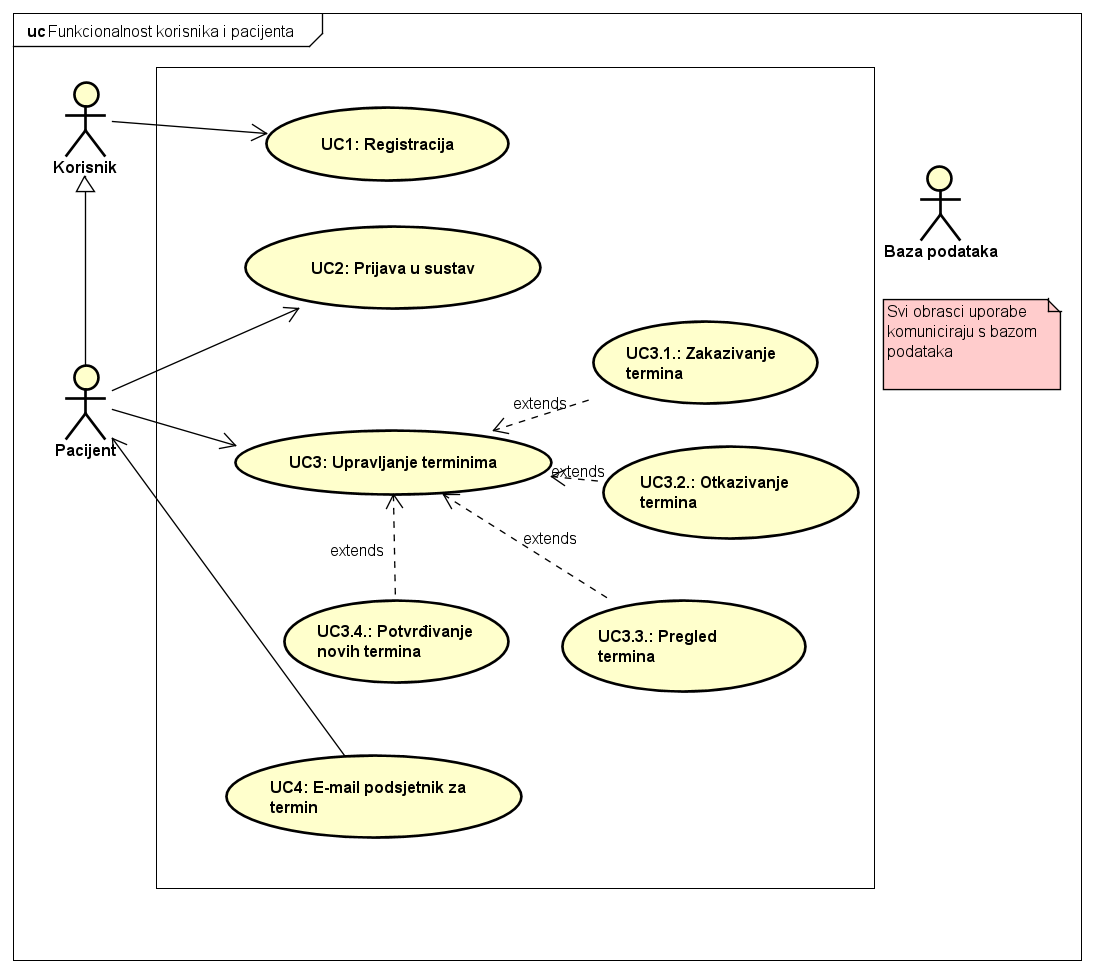
\includegraphics[scale=0.6]{slike/KorisnikIPacijent.PNG} %veličina slike u odnosu na originalnu datoteku i pozicija slike
						\centering
						\caption{Dijagram obrasca uporabe koji prikazuje funkcionalnost korisnika i pacijenta}
						\label{fig:promjene}
					\end{figure}
					
					\begin{figure}[H]
						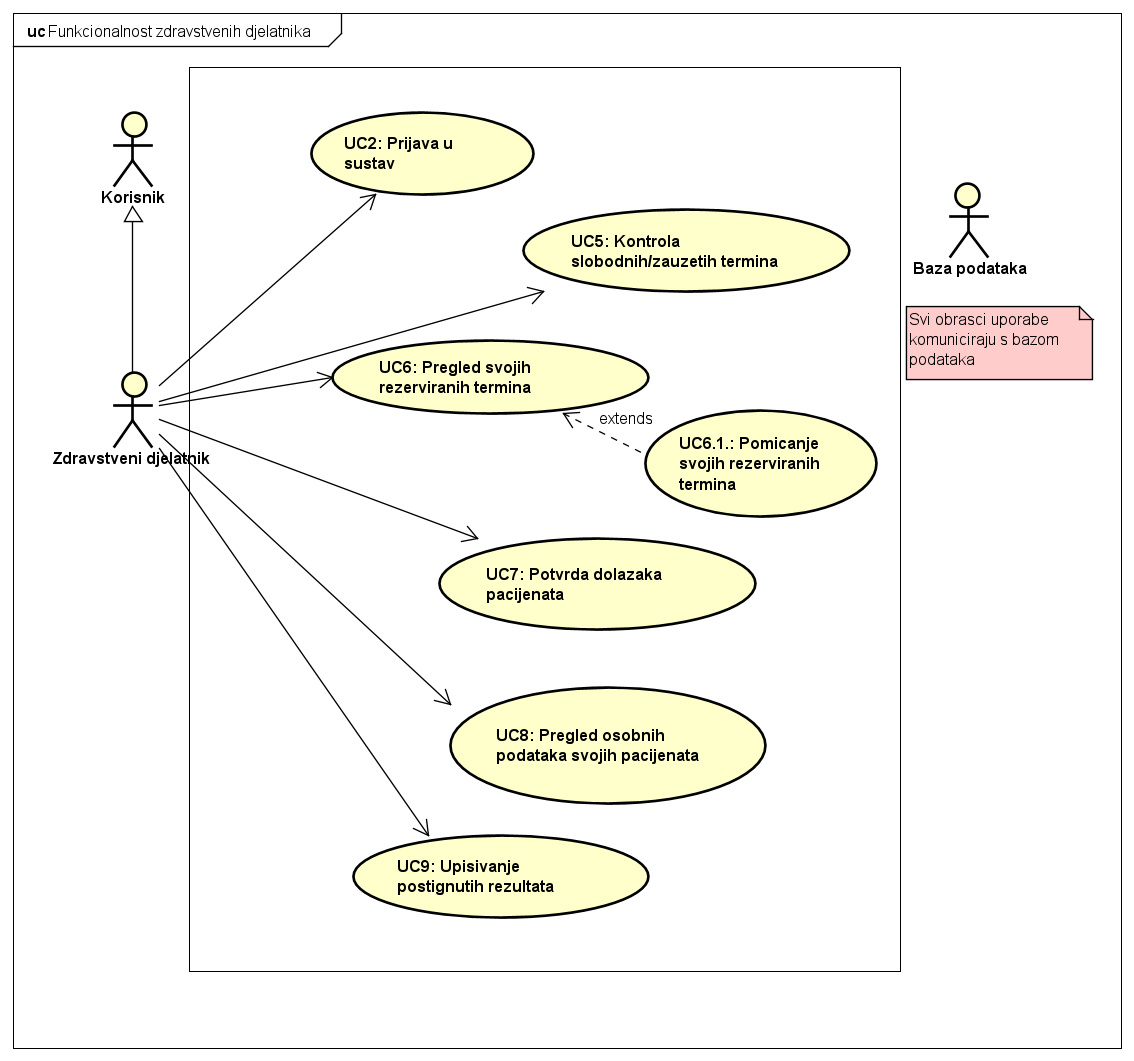
\includegraphics[scale=0.6]{slike/ZdravstveniDjelatnik.PNG} %veličina slike u odnosu na originalnu datoteku i pozicija slike
						\centering
						\caption{Dijagram obrasca uporabe koji prikazuje funkcionalnost zdravstvenih djelatnika}
						\label{fig:promjene}
					\end{figure}
					
					\begin{figure}[H]
						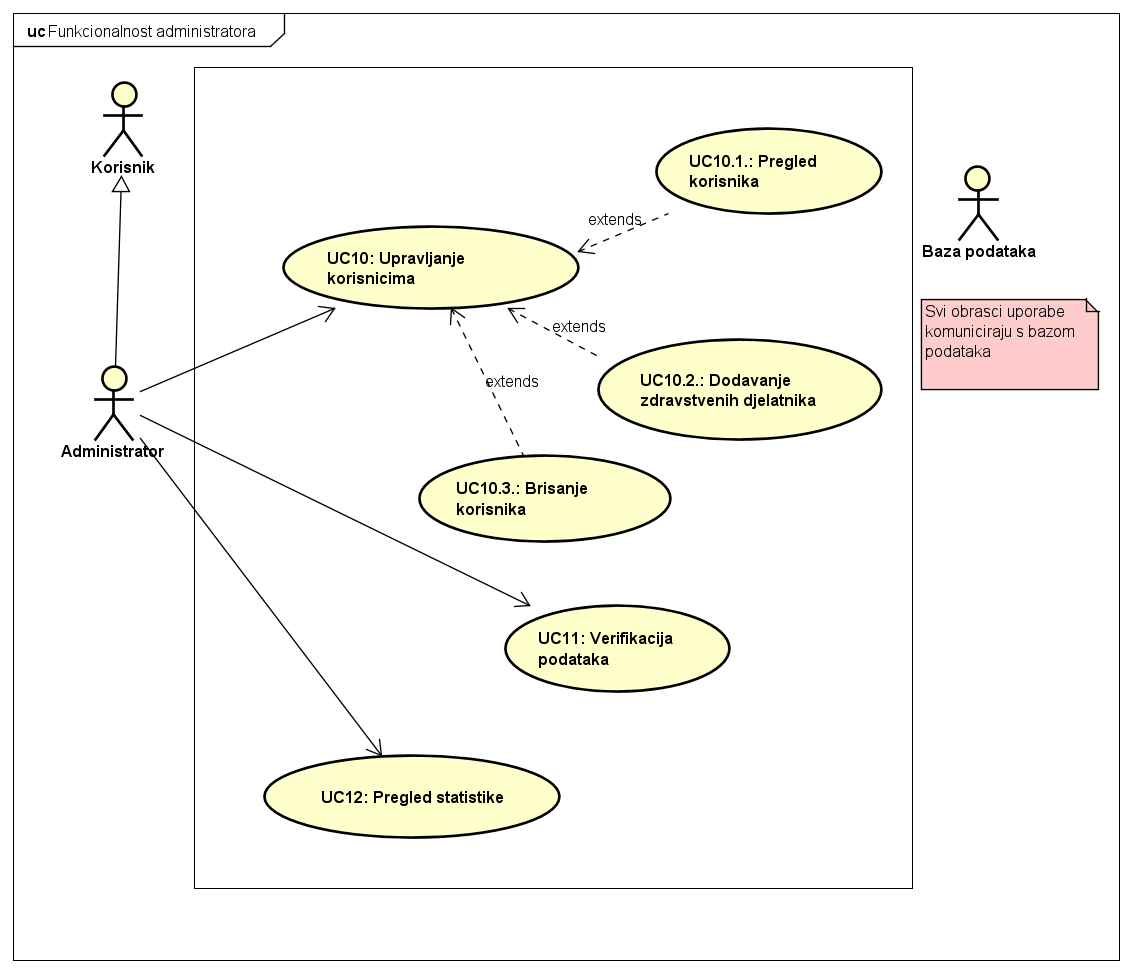
\includegraphics[scale=0.6]{slike/Administrator.PNG} %veličina slike u odnosu na originalnu datoteku i pozicija slike
						\centering
						\caption{Dijagram obrasca uporabe koji prikazuje funkcionalnost administratora}
						\label{fig:promjene}
					\end{figure}
				
			\subsection{Sekvencijski dijagrami}
				
				\textbf{\textit{dio 1. revizije}}\\
				
				\textit{Nacrtati sekvencijske dijagrame koji modeliraju najvažnije dijelove sustava (max. 4 dijagrama). Ukoliko postoji nedoumica oko odabira, razjasniti s asistentom. Uz svaki dijagram napisati detaljni opis dijagrama.}
				\eject
	
		\section{Ostali zahtjevi}
		
			\textbf{\textit{dio 1. revizije}}\\
		 
			 \textit{Nefunkcionalni zahtjevi i zahtjevi domene primjene dopunjuju funkcionalne zahtjeve. Oni opisuju \textbf{kako se sustav treba ponašati} i koja \textbf{ograničenja} treba poštivati (performanse, korisničko iskustvo, pouzdanost, standardi kvalitete, sigurnost...). Primjeri takvih zahtjeva u Vašem projektu mogu biti: podržani jezici korisničkog sučelja, vrijeme odziva, najveći mogući podržani broj korisnika, podržane web/mobilne platforme, razina zaštite (protokoli komunikacije, kriptiranje...)... Svaki takav zahtjev potrebno je navesti u jednoj ili dvije rečenice.}
			 
			 
			 
	